\documentclass[11pt,letterpaper]{article}
\usepackage{fullpage}
\usepackage{multicol}
\usepackage{amsmath}
\usepackage{amsfonts}
\usepackage{amssymb}
\usepackage{graphicx}
%\usepackage{pstricks, pst-node, pst-plot}

\newcommand{\ds}{\displaystyle}
\newcommand{\bv}{\mathbf}
\newcommand{\lv}{\langle}
\newcommand{\rv}{\rangle}

\begin{document}
\flushleft
\begin{multicols}{2}


\begin{large}\textbf{Math 115 Quiz 2: $\oint $ 1.6-1.8, 2.1 \\
Mon 27 September 2010}\end{large}

\textbf{Name:  }\underline{\hspace{35ex}}

\vspace{.5in}

\end{multicols}

\pagestyle{empty}


\flushleft

You have 15 minutes to complete this quiz.  Calculators are OK.  Eyes on your own paper and good luck!

\begin{enumerate}
\item  \textbf{Definitions/Concepts.} (1 pt each) Suppose that $\lim_{x\rightarrow 3}f(x)=7$.  Are the following statements true or false?  If a statement is true, explain how you know.  If a statement is false, give a counterexample.
\begin{enumerate} 
\item $\lim_{x\rightarrow 3}\left(xf(x)\right)=21$.  \textbf{TRUE}
\begin{eqnarray*}
 \lim_{x\rightarrow 3}\left(xf(x)\right) &=& \left(\lim_{x\rightarrow 3}x\right)\left(\lim_{x\rightarrow 3}f(x)\right) \\
&=& 3\cdot 7 \\
&=& 21.
\end{eqnarray*}

\vspace{.5pc}
\item If $g(3)=4$, then $\lim_{x\rightarrow 3}\left(f(x)+g(x)\right)=28$.  \textbf{FALSE}

\vspace{.5pc}
Suppose
\[g(x)=\left\{\begin{array}{ll}
               4 & \text{when }x=3 \\
               x & \text{when }x\neq 3.
              \end{array}\right.
\]
Then $\lim_{x\rightarrow 3}g(x)=3$.  Therefore
\begin{eqnarray*}
 \lim_{x\rightarrow 3}\left(f(x)+g(x)\right) &=& \lim_{x\rightarrow 3}f(x)+\lim_{x\rightarrow 3}g(x) \\
&=& 3+3 \\
&=& 6 \\
&\neq & 28.
\end{eqnarray*}
\textit{This problem was taken out of the Chapter 1 Review section and was not meant to have the plus sign.  However, the above solution illustrates why you should still not assume the limit of $g$ is 4 as $x$ approaches 3, even though $g(3)=4$.}

\vspace{.5pc}
\end{enumerate}

\item \textbf{Questions/Problems.} A ball is tossed into the air from a bridge, and its height, $y$ (in feet), above the ground $t$ seconds after it is thrown is given by 
\[y=f(t)=-16t^2+50t+36.\]
\begin{enumerate}
\item (1 pt) How high above the ground is the bridge? 

\vspace{.5pc}
The height of the bridge is given at the initial moment, when $t=0$.  So
\begin{eqnarray*}
 f(0) &=& -16(0)^2+50(0)+36 \\
&=& 36 \text{ ft.}
\end{eqnarray*}

\vspace{.5pc}
\item (1 pt) What is the average velocity of the ball for the first second?

\vspace{.5pc}
Compute the difference in height from the initial moment to the first second:
\begin{eqnarray*}
 f(1)-f(0) &=& 70-36 \\
&=& 34 \text{ ft/sec.}
\end{eqnarray*}

\vspace{.5pc}
\item (1 pt) Approximate the velocity of the ball at $t=1$ second.

\vspace{.5pc}
Look at the change in height at times close to $t=1$ second.
\begin{eqnarray*}
 \frac{f(1)-f(0.999)}{0.001} &=& 18.016 \\
 \frac{f(1)-f(0.9999)}{0.0001} &\approx & 18.002 \\
 \frac{f(1)-f(0.99999)}{0.00001} &\approx & 18.000 \\
 \frac{f(1.00001)-f(1)}{0.00001} &\approx & 18.000 \\
 \frac{f(1.0001)-f(1)}{0.0001} &\approx & 17.998 
\end{eqnarray*}
Conclude the velocity at $t=1$ second is approximately 18.000 ft/sec.

\vspace{.5pc}
\item (2 pts) Graph $f$, and determine the maximum height the ball reaches.  What is the velocity at the time the ball is at its peak?

\begin{center}
 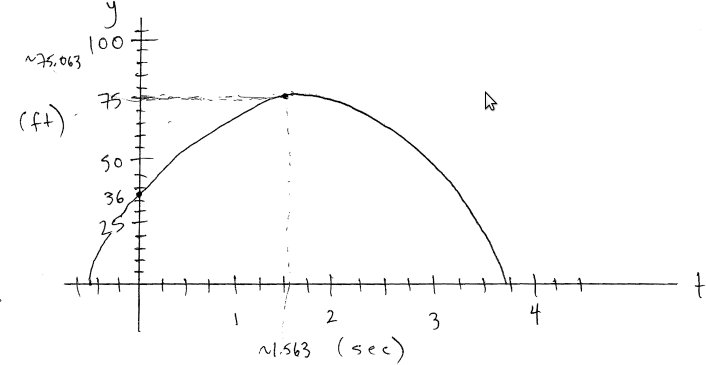
\includegraphics[scale=.4]{./115f10quiz2pic.jpg}
 % 115f10quiz2pic.jpg: 706x365 pixel, 72dpi, 24.91x12.88 cm, bb=0 0 706 365
\end{center}

The maximum height is approximately 75.063 ft.  The velocity at that height is 0 ft/sec.

\vspace{.5pc}
\item (1 pt) Use the graph to decide at what time, $t$, the ball reaches its maximum height.

\vspace{.5pc}
The ball reaches its maximum height at approximately 1.563 sec.

\vspace{.5pc}
\end{enumerate}

\item \textbf{Computations/Algebra.} (1 pt each) 
\begin{enumerate} 
\item Find $k$ so that the following function is continuous on any interval:
\[f(x)=\left\{\begin{array}{ll}
               kx & x\leq 3 \\
               5 & 3<x 
              \end{array}\right.\]
The function is continuous on any interval that does not contain 3, unless $k$ is assigned the appropriate value.  To make the function continuous at $x=3$, set $k\cdot (3)=5$, which implies $k=\frac{5}{3}$.

\vspace{.5pc}
\item Find $k$ so that the following function is continuous on any interval:
\[f(x)=\left\{\begin{array}{ll}
               kx & 0\leq x<2 \\
               3x^2 & 2\leq x 
              \end{array}\right.\]
As in part (a), set $k\cdot (2)=3(2)^2$.  Then $k=6$.

\vspace{.5pc}
\textit{The original quiz had a typo in this problem which has since been corrected.}
\end{enumerate}

\end{enumerate}

\end{document}


